\documentclass{beamer}
\usepackage{graphicx}
\usepackage{multirow}
\usepackage[utf8]{inputenc}
\usepackage[UKenglish]{babel}
\usepackage[UKenglish]{isodate}
\usepackage[style=authoryear]{biblatex}

\usetheme{PaloAlto}
\usecolortheme{orchid}
\beamertemplatenavigationsymbolsempty
\addbibresource{../dissertation/references.bib}
\author{Paulius Dilkas}
\title{Algorithm Selection for Maximum Common Subgraph}
\date{16th January 2018}
\institute{School of Computing Science, University of Glasgow}

\begin{document}
\maketitle

%\begin{frame}{Outline}
%\tableofcontents
%\end{frame}

\section{Algorithm selection}
\begin{frame}{Algorithm selection}
  \begin{definition}[\cite{DBLP:journals/ai/BischlKKLMFHHLT16}]
    Given a set $\mathcal{I}$ of problem instances, a space of algorithms
    $\mathcal{A}$, and a performance measure $m \colon \mathcal{I} \times
    \mathcal{A} \to \mathbb{R}$, the \emph{algorithm selection problem} is to
    find a mapping $s \colon \mathcal{I} \to \mathcal{A}$ that optimises
    $\mathbb{E}[m(i, s(i))]$.
  \end{definition}
  \pause
  \centering{\textsc{Llama} \parencite{kotthoff_llama_2013}}
  \begin{figure}
    \centering
    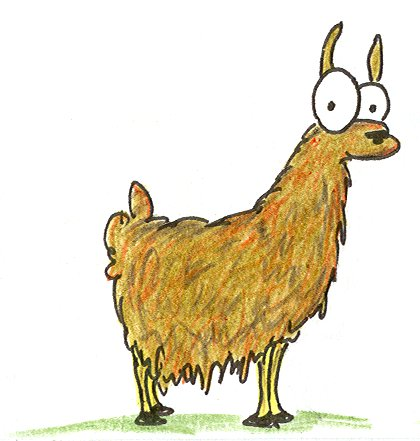
\includegraphics[scale=0.5]{llama.jpg}
  \end{figure}
\end{frame}

\section{Algorithms}
\begin{frame}{Algorithms}
  \begin{itemize}
  \item \textsc{McSplit}, $\textsc{McSplit}\downarrow$
    \begin{itemize}
    \item \parencite{DBLP:conf/ijcai/McCreeshPT17}
    \end{itemize}
  \item clique encoding
    \begin{itemize}
    \item \parencite{DBLP:conf/cp/McCreeshNPS16}
    \end{itemize}
  \item $k\downarrow$
    \begin{itemize}
    \item \parencite{DBLP:conf/aaai/HoffmannMR17}
    \end{itemize}
  \end{itemize}
\end{frame}

\section{Labelling}
\begin{frame}{Labelling}
  Data from \cite{foggia2001-2, DBLP:journals/prl/SantoFSV03} (81400 pairs
  of graphs)
  \pause
  \begin{definition}
    A \emph{vertex-labelled graph} is a 3-tuple $G = (V, E, \mu)$, where $\mu
    \colon V \to \{ 0, \dots, N - 1 \}$ is a vertex labelling function, for some
    $N \in \mathbb{N}$.
  \end{definition}
  \pause
  \begin{definition}
    A graph $G = (V, E, \mu)$ is said to have a \emph{$p\%$ (vertex) labelling} if
    \[ N = \max \left\{ 2^n : n \in \mathbb{N},\, 2^n < \left\lfloor \frac{p}{100\%}
          \times |V| \right\rfloor \right\}. \]
  \end{definition}
\end{frame}

\begin{frame}{Labelling}
  \begin{definition}
    A graph $G = (V, E, \mu)$ is said to have a \emph{$p\%$ (vertex) labelling} if
    \[ N = \max \left\{ 2^n : n \in \mathbb{N},\, 2^n < \left\lfloor \frac{p}{100\%}
          \times |V| \right\rfloor \right\}. \]
  \end{definition}
  \begin{itemize}
  \item 5\% labelling - 20 vertices per label on average
  \item 50\% labelling - 2 vertices per label on average
    \pause
  \item Typical values explored: 33\%, 50\%, 75\%
    \pause
  \item In my data: 5\%, 10\%, 15\%, 20\%, 25\%, 33\%, 50\%
    \pause
  \item 3 subproblems
    \begin{itemize}
    \item no labels
    \item vertex labels
    \item vertex and edge labels
    \end{itemize}
  \end{itemize}
\end{frame}

%\begin{frame}{Distribution of vertices per label}
%  \begin{figure}
%    \centering
%    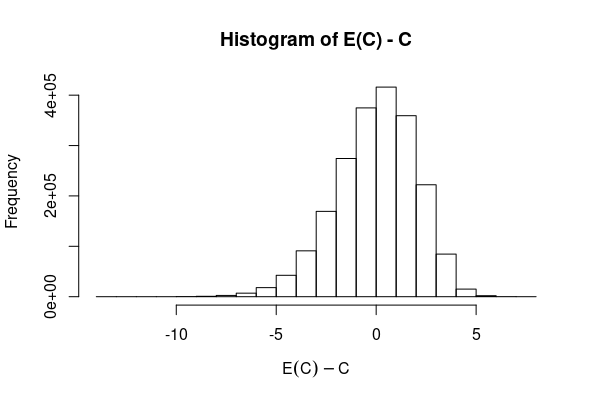
\includegraphics[scale=0.4]{../dissertation/images/labelling_histogram.png}
%  \end{figure}
%  For each graph and label
%  \begin{itemize}
%  \item $C$ is the number of vertices with that label
%  \item $E(C)$ is the number we would expect from a (discrete) uniform distribution
%  \end{itemize}
%\end{frame}

\section{Features}
\begin{frame}{Features (34 in total)}
  1--8 are from \cite{DBLP:conf/lion/KotthoffMS16}
  \begin{enumerate}
  \item number of vertices
  \item number of edges
  \item mean/max degree
  \item density
  \item mean/max distance between pairs of vertices
  \item number of loops
  \item proportion of vertex pairs with distance $\ge$ 2, 3, 4
  \item connectedness
    \pause
  \item standard deviation of degrees
  \item labelling percentage
    \pause
  \item ratios of features 1--5
  \end{enumerate}
\end{frame}

\section{Random forests}

\begin{frame}{Random forests \parencite{DBLP:journals/ml/Breiman01}}
  \begin{figure}
    \centering
    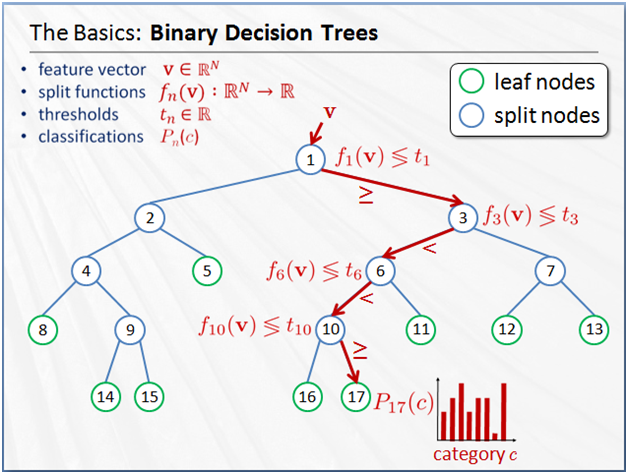
\includegraphics[scale=0.5]{random_forests_2.png} \\
    {\tiny\color{gray}Source: Tae-Kyun Kim \& Bjorn Stenger, Intelligent Systems and Networks (ISN) Research Group,\\[-7pt] Imperial College London}
  \end{figure}
\end{frame}

\begin{frame}{Random forests \parencite{DBLP:journals/ml/Breiman01}}
  \begin{figure}
    \centering
    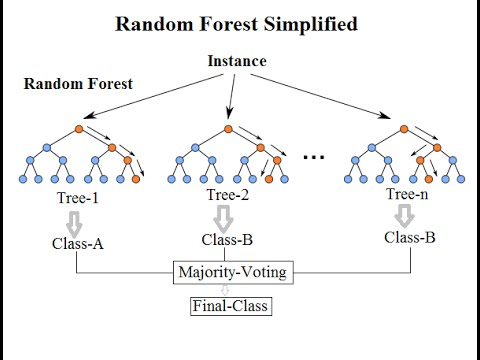
\includegraphics[scale=0.5]{rand-forest-1.jpg} \\
    {\tiny\color{gray}Source: Random Forests(r), Explained, Ilan Reinstein, KDnuggets}
  \end{figure}
\end{frame}

\section{Results}

\begin{frame}{Results}
  \begin{figure}
    \centering
    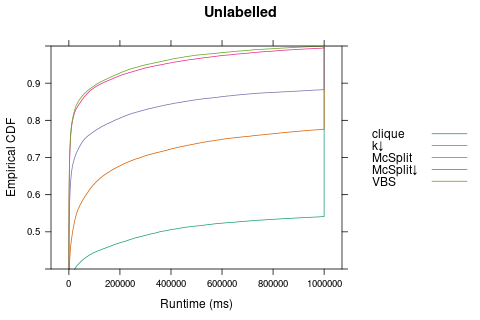
\includegraphics[width=\textwidth]{../dissertation/images/ecdf_unlabelled.png}
  \end{figure}
\end{frame}

\begin{frame}{Results (27\%)}
  \begin{figure}
    \centering
    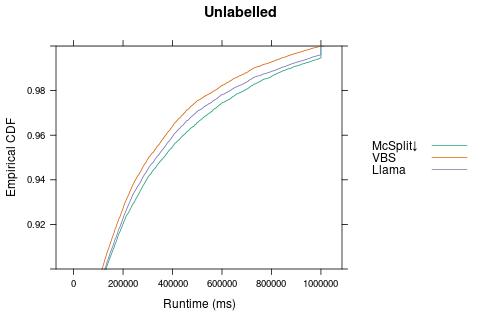
\includegraphics[width=\textwidth]{../dissertation/images/ecdf_unlabelled_llama.png}
  \end{figure}
\end{frame}

\begin{frame}{Results}
  \begin{figure}
    \centering
    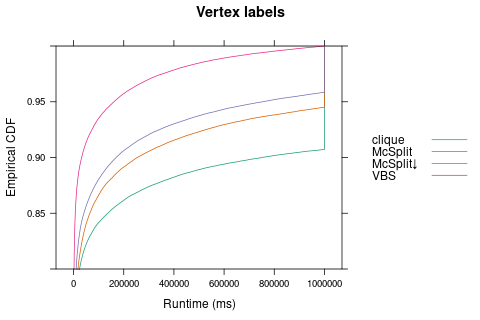
\includegraphics[width=\textwidth]{../dissertation/images/ecdf_vertex_labels.png}
  \end{figure}
\end{frame}

\begin{frame}{Results (86\%)}
  \begin{figure}
    \centering
    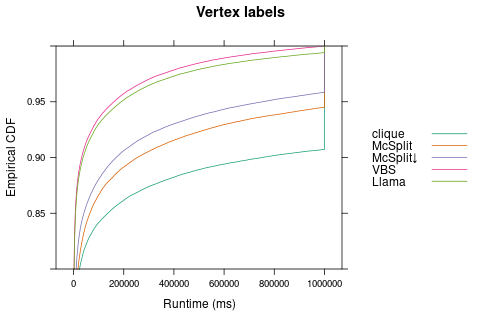
\includegraphics[width=\textwidth]{../dissertation/images/ecdf_vertex_labels_llama.png}
  \end{figure}
\end{frame}

\begin{frame}{Results}
  \begin{figure}
    \centering
    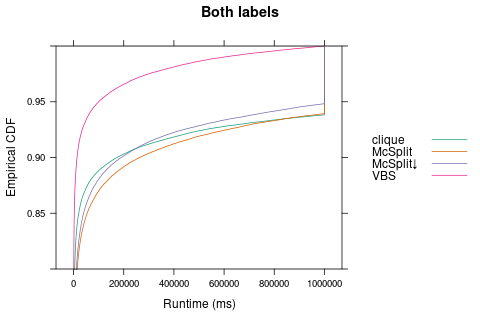
\includegraphics[width=\textwidth]{../dissertation/images/ecdf_both_labels.png}
  \end{figure}
\end{frame}

\begin{frame}{Results (88\%)}
  \begin{figure}
    \centering
    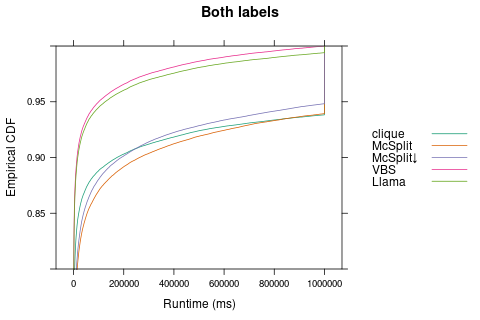
\includegraphics[width=\textwidth]{../dissertation/images/ecdf_both_labels_llama.png}
  \end{figure}
\end{frame}

%\begin{frame}{Other observations}
%  \begin{itemize}
%  \item Most important features
%    \begin{itemize}
%    \item labelling percentage
%    \item standard deviation of degrees (for both graphs)
%    \end{itemize}
%  \end{itemize}
%\end{frame}

\begin{frame}{Errors}
  \begin{itemize}
  \item Out-of-bag error
  \item For each algorithm
    \begin{itemize}
    \item $1 - \text{recall}$
    \end{itemize}
  \end{itemize}
  \begin{definition}
    For an algorithm $A$, \emph{recall} (sensitivity) is
    \[ \frac{\text{the number of instances that were correctly predicted as
          $A$}}{\text{the number of instances where $A$ is the correct
          prediction}}. \]
  \end{definition}
\end{frame}

\begin{frame}{Errors (\%)}
  \centering
  \begin{tabular}{l | c c c}
    \multirow{2}{*}{Error} & \multicolumn{3}{c}{Labelling} \\
                           & no & vertex & both \\
    \hline
    out-of-bag & 17 & 13 & 14 \\
    clique & 30 & 8 & 7 \\
    \textsc{McSplit} & 29 & 22 & 29 \\
    $\textsc{McSplit}\downarrow$ & 11 & 11 & 11 \\
    $k\downarrow$ & 80 & &
  \end{tabular}
\end{frame}

\begin{frame}{Convergence of errors for unlabelled graphs}
  \begin{figure}
    \centering
    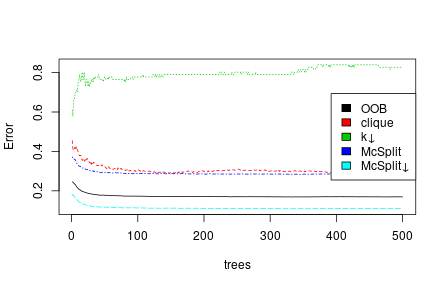
\includegraphics[scale=0.5]{../dissertation/images/unlabelled_forest_errors.png}
  \end{figure}
\end{frame}

\section{What happens when labelling changes?}
\begin{frame}{What happens when labelling changes?} % total runtime is equivalent
  \begin{columns}
    \begin{column}{0.5\textwidth}
      \begin{figure}
        \centering
        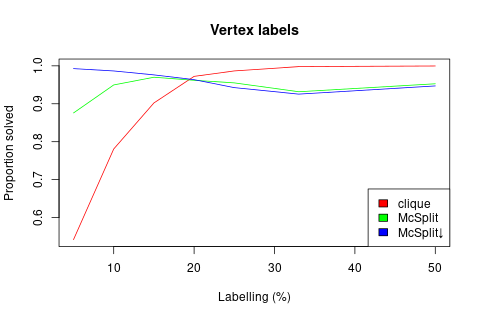
\includegraphics[width=\textwidth]{../dissertation/images/vertex_labels_linechart.png}
        \visible<2>{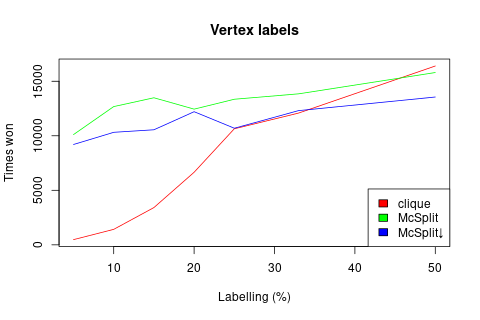
\includegraphics[width=\textwidth]{../dissertation/images/vertex_labels_linechart3.png}}
      \end{figure}
    \end{column}
    \begin{column}{0.5\textwidth}
      \begin{figure}
        \centering
        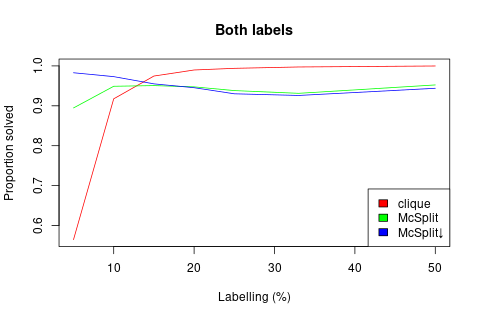
\includegraphics[width=\textwidth]{../dissertation/images/both_labels_linechart.png}
        \visible<2>{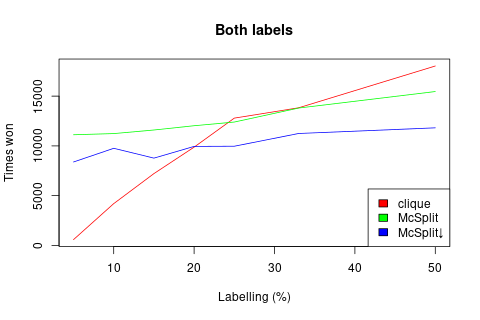
\includegraphics[width=\textwidth]{../dissertation/images/both_labels_linechart3.png}}
      \end{figure}
    \end{column}
  \end{columns}
\end{frame}

\section{Future work}
\begin{frame}{Future work}
  \begin{itemize}
  \item Relationships between clique algorithm's performance and properties of
    the association graph
  \item How the association graph changes after making a decision
  \item Can $k\downarrow$ and clique work together?
  \end{itemize}
\end{frame}

%\begin{frame}{Margins}
%  \begin{definition}
%    Let $c_1, \dots, c_n$ be $n$ classes and let $p$ be a data point that belongs
%    to class $c_p$. Let $v_1, \dots, v_n$ denote the number of votes for each
%    class when given $p$ as input. The \emph{margin} of $p$ is
%    \[ \frac{v_p}{\sum_{i=1}^n v_i} - \max_{i \ne p} \frac{v_i}{\sum_{j=1}^n v_j}, \]
%    which is a number in $[-1, 1]$.
%  \end{definition}
%\end{frame}

\end{document}